\section{اصلاح پارامتر‌های  استند چهارپره}\label{parameeter_estimation_section}
در بخش
\ref{spacestate}
فرم فضای حالت استند چهارپره استخراج شد و  در بخش
\ref{quadall3}
شبیه‌سازی استند چهارپره انجام شد.
در این بخش، با استفاده از شبیه‌سازی کانال‌های مختلف چهارپره در محیط سیمولینک و داده‌های خروجی  از استند چهارپره، پارامترهای استند چهارپره اصلاح می‌شوند.

برای اصلاح پارامترهای استند چهارپره از جعبه‌ابزار
\lr{Parameter Estimator}
موجود در محیط سیمولینک
استفاده شده‌است.
این جعبه ابزار با استفاده از داده‌های وضعیت استند در واقعیت و داده‌های وضعیت استند در شبیه‌سازی سیمولینک، اقدام به اصلاح پارامترهای موجود در شبیه‌سازی می‌کند، به‌صورتی که وضعیت استند در شبیه‌سازی تا حد ممکن به  وضعیت استند در واقعیت نزدیک کند.

%\newline

	\hspace*{.5cm}
\begin{figure}[H]

	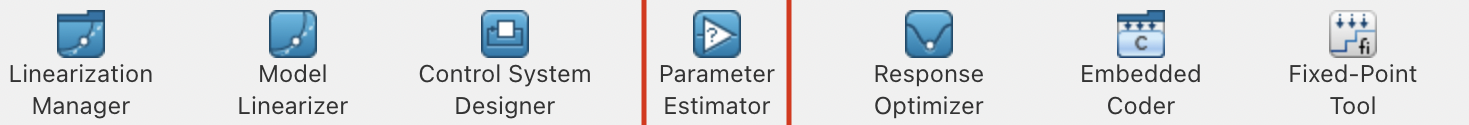
\includegraphics[width=12cm]{../Figures/QuadSimulation/ParameterEstimation/PS_icon.png}
	\centering
	\caption{نماد جعبه‌ابزار
	\lr{Parameter Estimator}
در سیمولینک}
\end{figure}
در شکل
\ref{PS}
نمایی از این جعبه‌ابزار آورده شده‌است.





	\hspace*{-0.5cm}
\begin{figure}[H]
	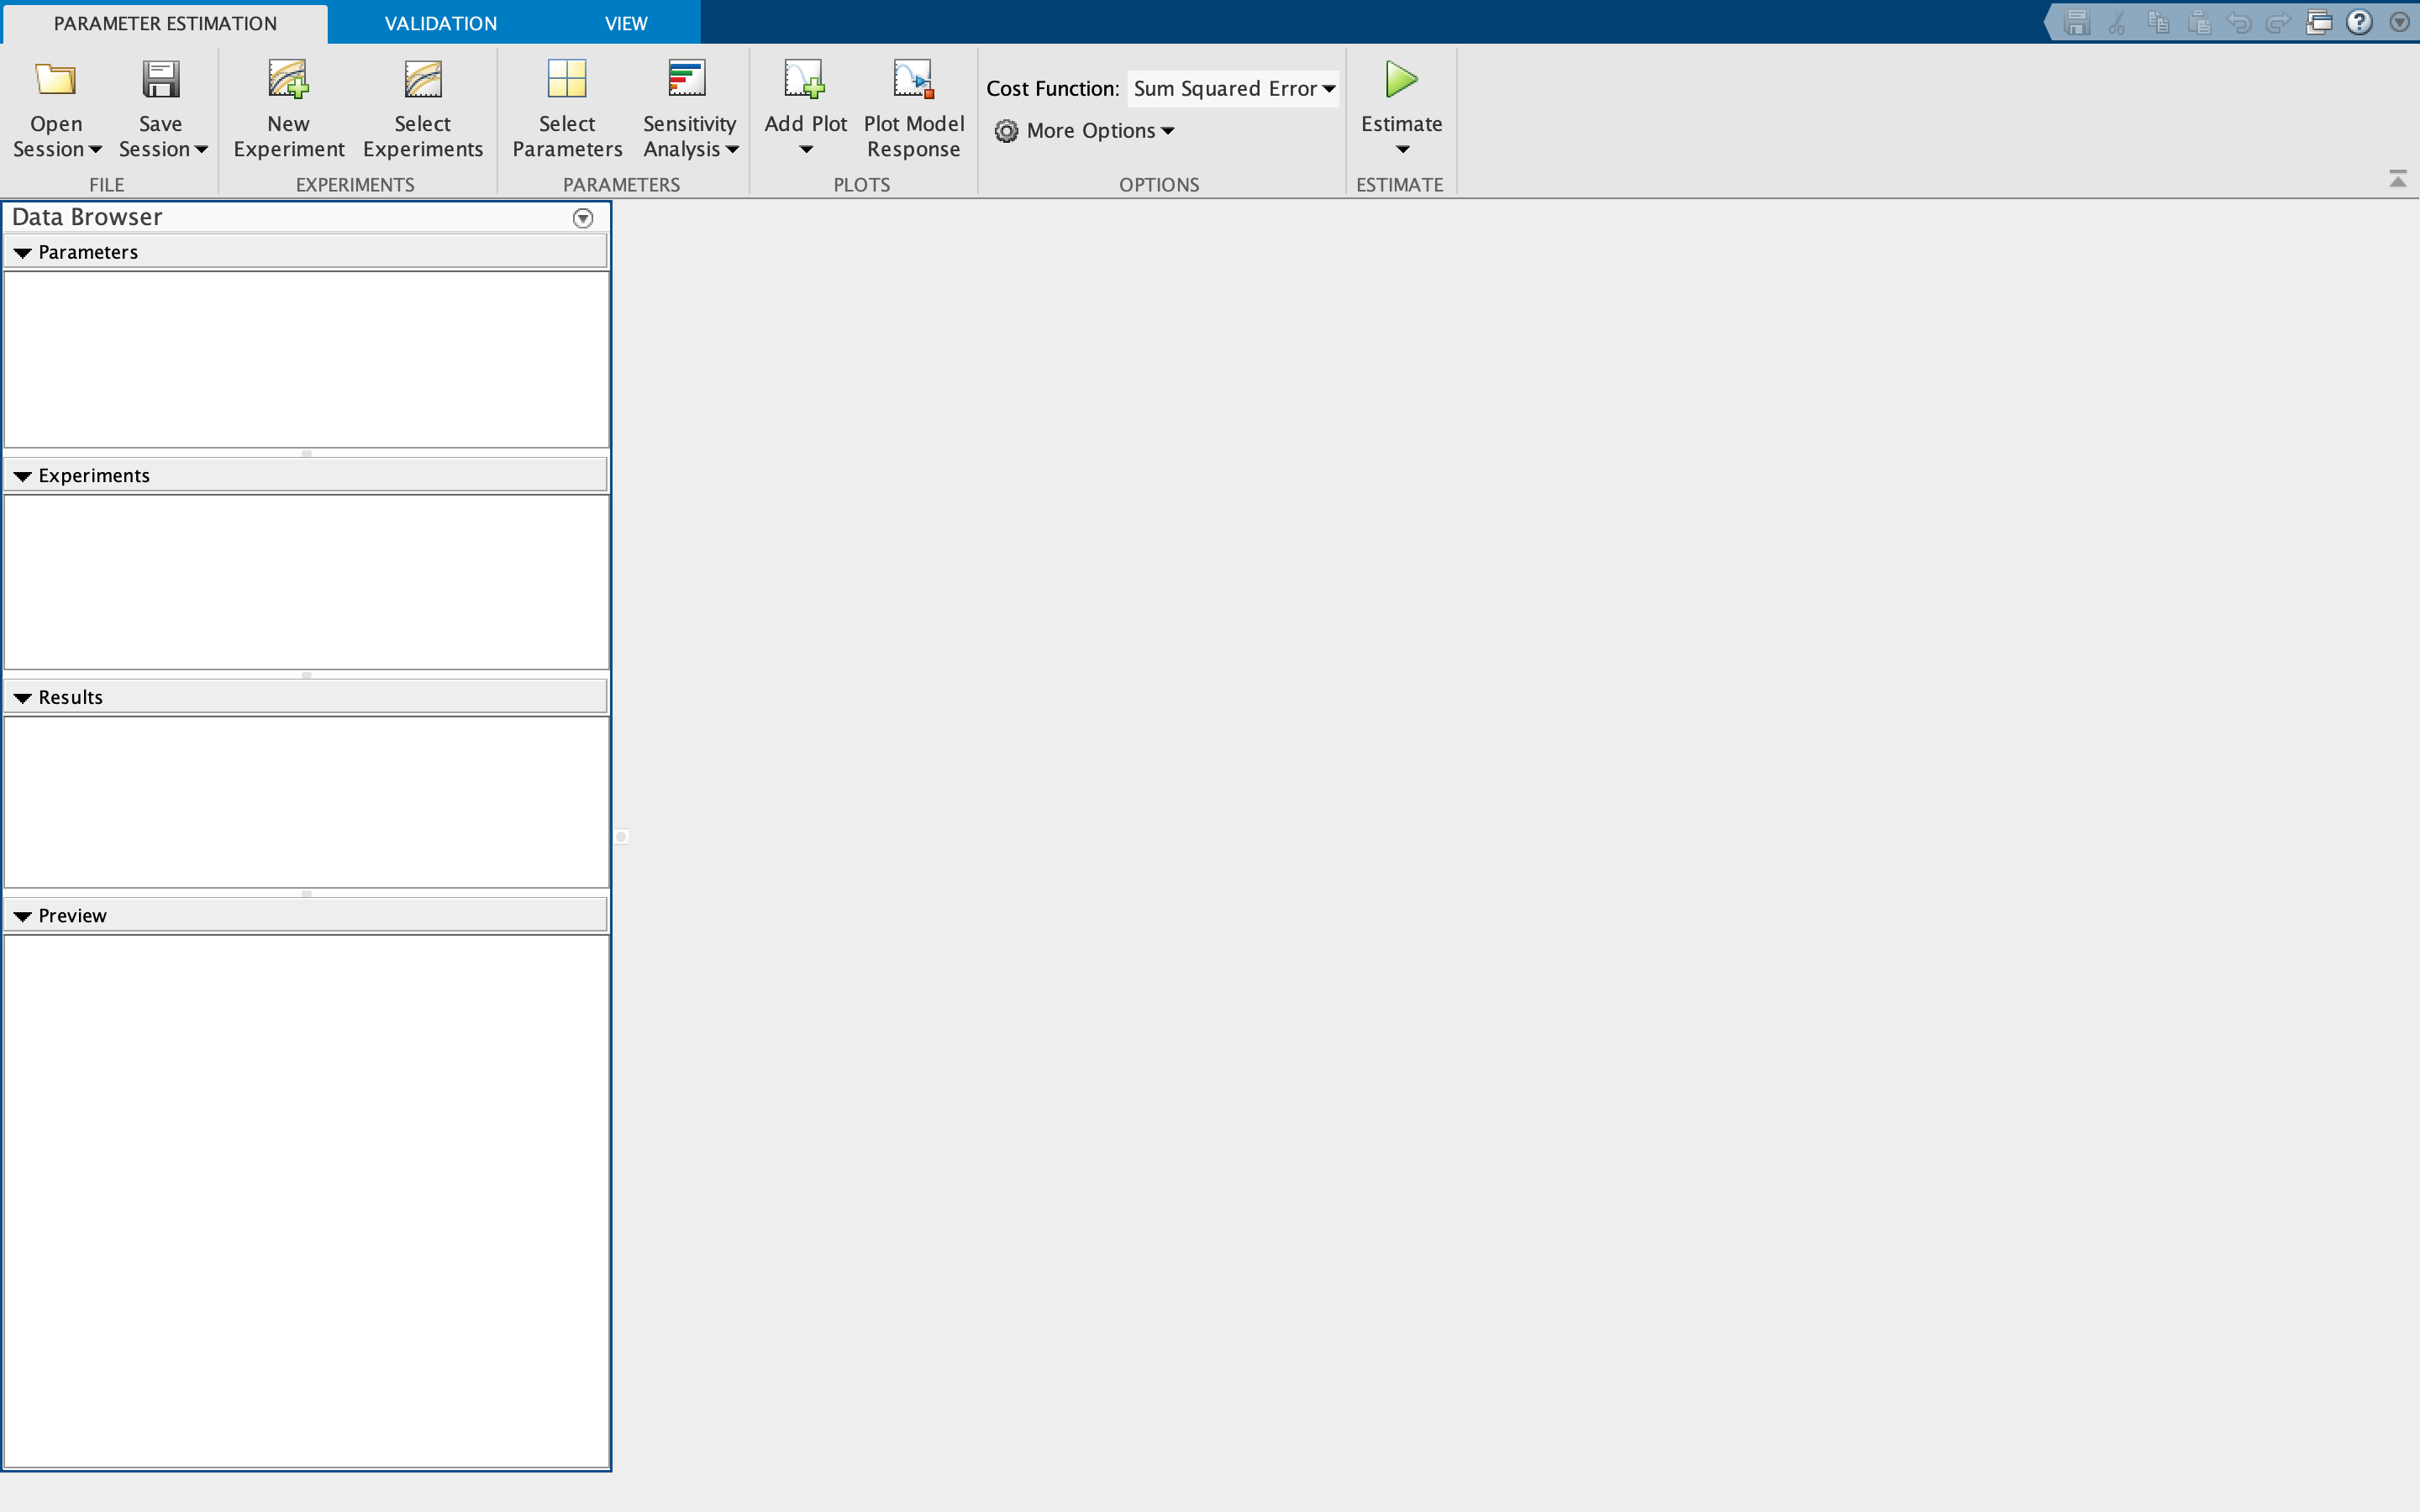
\includegraphics[width=12cm]{../Figures/QuadSimulation/ParameterEstimation/PS_app.png}
	\centering
	\caption{جعبه‌ابزار
	\lr{Parameter Estimator}}
	\label{PS}
\end{figure}

